% !TEX options=--shell-escape
\documentclass[12pt]{article}
\usepackage[utf8]{inputenc}
\usepackage{lipsum}
\usepackage{afterpage}
\usepackage{mathtools}
\usepackage{xcolor}
\usepackage[12pt]{extsizes}
\usepackage[english,russian]{babel}
\usepackage{cite}
\usepackage{minted}
\usepackage{amsmath, esint, setspace, fancyhdr, amsfonts, bookmark, blindtext}
\usepackage{graphicx}
\usepackage{subfigure}
\usepackage{titlesec}

\graphicspath{{Figures/}}
\DeclareGraphicsExtensions{.pdf,.png,.jpg}
\usemintedstyle{tango}
\definecolor{dhscodebg}{rgb}{0.95,0.95,0.95}


\setlength{\textheight}{8in}
\setlength{\textwidth}{6.6in}
\setlength{\headheight}{0in}
\setlength{\headsep}{0.2in}
\setlength{\topmargin}{0in}
\setlength{\oddsidemargin}{0in}
\setlength{\evensidemargin}{0in}
\setlength{\parindent}{.3in}

\doublespacing
\renewcommand{\baselinestretch}{1.4} 
\newcommand{\RNumb}[1]{\uppercase\expandafter{\romannumeral #1\relax}}

\begin{document}
\begin{titlepage}

\begin{center}
Санкт-Петербургский политехнический университет Петра Великого\\
Институт прикладной математики и механики\\
Кафедра прикладной математики\\
\end{center}


\vspace{2.5cm}

\begin{center}
{\large {\bfseries СВОДНЫЙ ОТЧЕТ}}\\

\bigskip \bfseries{Тема:} {\bfseries \emph{Многомерные распределения.\\ Оценки характеристик распределений}}
\end{center}

\vspace{1.5cm}

\begin{flushleft}
Направление: 01.03.02 Прикладная математика и информатика

\vspace{1.5cm}

Выполнил студент гр. 33631/4 \hfill{Камалетдинова Ю.} \\ 

\vspace{0.5cm} Преподаватель \hfill{Баженов А.}
\vspace{1cm}

\end{flushleft}

\vspace{2.7cm}

\begin{center}
Санкт-Петербург\\
2019
\end{center}

\end{titlepage}

\newcommand{\threeimage}[4]{
\begin{figure}[h!]  
    \centering 
    \subfigure[]{
        \includegraphics[width=0.3\linewidth, height=0.25\linewidth]{#1} 
        \label{fig:f_ #1} }  
        %\hspace{4ex}
    \subfigure[]{
    \includegraphics[width=0.3\linewidth, height=0.25\linewidth]{#2} 
    \label{fig:f_ #2} }
   % \hspace{4ex}
    \subfigure[]{ 
        \includegraphics[width=0.3\linewidth, height=0.25\linewidth]{#3} 
        \label{fig:f_ #3} }  
    \caption{Выборки из #4 объемом: 
    \subref{fig:f_ #1} 20; 
    \subref{fig:f_ #2} 60; 
    \subref{fig:f_ #3} 100} 
    \label{fig:f_ #1#2#3}
\end{figure}}

\newcommand{\triplethreeimage}[4]{
\begin{figure}[h!]  
    \centering 
    \subfigure[]{
        \includegraphics[width=.83\linewidth, height=.3\linewidth]{#1} 
        \label{fig:f_ #1} }\\  
    %\hspace{4ex}
    \subfigure[]{
        \includegraphics[width=.83\linewidth, height=.3\linewidth]{#2} 
        \label{fig:f_ #2} }\\
    %\hspace{4ex}
    \subfigure[]{ 
        \includegraphics[width=.83\linewidth, height=.3\linewidth]{#2} 
        \label{fig:f_ #3} }  
    \caption{Для выборок из #4 объемом: 
    \subref{fig:f_ #1} 20; 
    \subref{fig:f_ #2} 60; 
    \subref{fig:f_ #3} 100} 
    \label{fig:f_ #1#2#3}
\end{figure}}


\tableofcontents
\addtocontents{toc}{~\hfill\par}
\vfill ~
\setcounter{section}{0}


%%%%%%%%%%%%%%%%%%%%%%%%%%%%%%%%%%%%%%%%%%

\newpage 
\section*{Постановка задачи}
\addcontentsline{toc}{section}{Постановка задачи}


\indent{\indentРассматривается один из методов точечной оценки характеристик распределения. Требуется сгенерировать выборку объемом $n = 100$ элементов для нормального распределения $N(x; 0, 1)$ и оценить по ней параметры $\mu$ и $\sigma$ нормального распределения методом максимального правдоподобия. В качестве основной гипотезы $H_0$ будем считать, что сгенерированное распределение имеет вид $N(x; \hat{\mu}, \hat{\sigma})$. Проверить гипотезу, используя критерий согласия $\chi^2$. В качестве уровня значимости взять $\alpha = 0.05$. Привести таблицу вычислений $\chi^2$.}


%%%%%%%%%%%%%%%%%%%%%%%%%%%%%%%%%%%%%%%%%%

\section*{Описание алгоритма}
\addcontentsline{toc}{section}{Описание алгоритма}
\subsection*{Метод максимального правдоподобия}
\indent{\indent Пусть $x_1, \ldots, x_n$ –– случайная выборка из распределения с плотностью вероятности $f(x; \theta)$. Функцией правдоподобия (ФП) назовем совместную плотность вероятности независимых случайных величин $x_1, \ldots, x_n$, рассматриваемую как функцию неизвестного параметра $\theta$}

\begin{equation}
	L(x_1, \ldots, x_n; \theta) = f(x_1; \theta)f(x_2; \theta)\ldots f(x_n; \theta)
	\label{eq_7:1}
\end{equation}

\indent{ Оценкой максимального правдоподобия $\hat\theta_{\text{МП}}$ будем называть такое значение , для которого из множества допустимых значений параметра $\theta$ ФП имеет наибольшее значение при заданных $x_1, \ldots, x_n$}

\begin{equation}
	\hat\theta_{\text{МП}} = arg \; max \; L(x_1, \ldots, x_n; \theta)
	\label{eq_7:2}
\end{equation}

\indent{ Если функция правдоподобия дважды дифференцируема, ее стационарные значения задаются корнями уравнения}

\begin{equation}
	\frac{\partial{L(x_1, \ldots, x_n; \theta)}}{\partial{\theta}} = 0
	\label{eq_7:3}
\end{equation}

Запишем условие локального максимума $\overline{\theta}$

\begin{equation}
	\frac{\partial^2 L}{\partial \theta^2} (x_1, \ldots, x_n; \overline{\theta}) 
	< 0
	\label{eq_7:4}
\end{equation}
Наибольший локальный максимум будет являться решением задачи \eqref{eq_7:2}. 

\indent{ Мы будем искать максимум логарифма функции правдоподобия в виду того, что он имеет максимум в одной точке с функцией правдоподобия}

\begin{equation}
	\frac{\partial \ln L}{\partial \theta} \text{, если $L > 0$,}
	\label{eq_7:5}
\end{equation}
и будем решать уравнение правдоподобия

\begin{equation}
    \frac{\partial \ln  L}{\partial \theta} = 0
    \label{eq_7:6}
\end{equation}

\indent{ Для проверки гипотезы о характере распределения воспользуемся критерием $\chi^2$ для случая, когда параметры распределения известны. Пусть $H_0$ –– гипотеза о генеральном законе распределения, $H_1$ –– гипотеза о справедливости одного из конкурирующих законов распределений. Разобьем генеральную совокупность на $k$ непересекающихся подмножеств $\Delta_1, \ldots, \Delta_k$ при условиях}

\begin{equation}
    p_i = P(X \in \Delta_i), \; i = \overline{1,k}\;; \;\; \sum_{i=1}^{k} p_i = 1
    \label{cond_7:1}
\end{equation}

\indent{ Положим $n_i$ –– частота попадания выборочного элемента в подмножество $\Delta_i$. За меру отклонения выборочного распределения от гипотетического примем величину}

\begin{equation}
    Z = \sum_{i=1}^{k}c_i \left(\frac{n_i}{n} - p_i\right)^2,
    \label{eq_7:7}
\end{equation}
где $\frac{n_i}{n}$ –– относительные частоты, $c_i$ –– некие положительные числа (веса). В качестве весов К. Пирсоном были взяты числа $c_i = \frac{n}{p_i}$. Получаем статистику критерия хи-квадрат К. Пирсона

\begin{equation}
    \chi^2 = \sum_{i=1}^{k}\frac{n}{p_i} \left(\frac{n_i}{p} - p_i\right)^2 = \sum_{i=1}^{k}\frac{(n_i - np_i)^2}{np_i}
    \label{eq_7:8}
\end{equation}

\indent{ По теореме К. Пирсона из пособия \cite{ms_1} статиcтика критерия $\chi^2$ асимптотически распределена по закону $\chi^2$ с $k - 1$ степенями свободы}

\indent{ Формулы \eqref{eq_7:1} –– \eqref{eq_7:8} и определения взяты из источника \cite{ms_1}}

%%%%%%%%%%%%%%%%%%%%%%%%%%%%%%%%%%%%%%%%%%

\section*{Реализация}
\addcontentsline{toc}{section}{Реализация}
\indent{\indentДля выполнения поставленной задачи будем пользоваться библиотеками для языка Python: \textit{numpy, scipy} -- расчеты, законы распределения вероятностей; \textit{matplotlib, seaborn} -- визуализация результатов. Ход работы:}
\begin{itemize}
    \item Генерируем выборку из распределения $N(x; 0, 1)$ объемом $n = 100$ 
    \item Запишем выражение для логарифма функции правдоподобия:
    \begin{equation}
    	\ln L = -\frac{n}{2} \ln 2\pi - \frac{n}{2} \ln(\sigma^2) - \frac{1}{2\sigma^2}\sum_{i=1}^{n}(x_i - \mu)^2
    	\label{eq_7:9}
    \end{equation}
    \item Получим два уравнения правдоподобия:
    \begin{equation}
    	\begin{cases}
    		\displaystyle \frac{\partial \ln L}{\partial \mu} = \frac{1}{\sigma^2}\sum_{i=1}^{n}(x_i - \hat \mu) = \frac{n}{\sigma^2}(\overline x - \hat m) = 0 \\
    		\displaystyle \frac{\partial \ln L}{\partial(\sigma^2)} = -\frac{n}{\hat \sigma^2} + \frac{1}{2(\hat \sigma^2)^2} \sum_{i=1}^{n}(x_i - \hat \mu)^2 = \frac{n}{2(\hat \sigma^2)^2} \left[\frac{1}{n} \sum_{i=1}^{n}(x_i - \hat \mu)^2 - \hat \sigma^2 \right] = 0
    	\end{cases}
    	\label{eq_7:10}
    \end{equation}
    \item Из уравнений \eqref{eq_7:10} получили, что выборочное среднее $\overline x$ –– оценка максимума правдоподобия математического ожидания: $\hat \mu_{\text{МП}} = \overline x$, а выборочная дисперсия \\ $s^2 = \frac{1}{n}\sum_{i=1}^{n}(x_i - \overline x^2)$ –– оценка максимума правдоподобия генеральной дисперсии $\hat \sigma^2_{\text{МП}} = s^2$
\end{itemize}

\indent{ Опишем порядок работы для проверки гипотезы о нормальности распределения по методу хи-квадрат}
\begin{itemize}
    \item Найдем квантиль $\chi^2_{1 - \alpha}(k - 1)$, где $\alpha = 0.05$ –– уровень значимости, $k = 1 + 3.3 \ln n = 16$ –– число подмножеств разбиения генеральной совокупности, вычисляемое по формуле Старджесса из источника \cite{ms_1}
    \item Вычисляем выборочное значение статистики хи-квадрат по формуле
    \begin{equation}
        \chi^2_B = \sum_{i=1}^{k}\frac{(n_i - np_i)^2}{np_i}
        \label{eq_7:11}
    \end{equation}
    \item Сравниваем $\chi^2_B$ и $\chi^2_{1 - \alpha}(k - 1)$
    \begin{itemize}
        \item Если $\chi^2_B < \chi^2_{1 - \alpha}(k - 1)$, то гипотеза $H_0$ на этапе проверки принимается
        \item Если $\chi^2_B \ge \chi^2_{1 - \alpha}(k - 1)$, то гипотеза $H_0$ отвергается, выбирается одно из альтернативных распределений и процедура проверки повторяется
    \end{itemize}
\end{itemize}

%%%%%%%%%%%%%%%%%%%%%%%%%%%%%%%%%%%%%%%%%%

\newpage
\section*{Результат}
\addcontentsline{toc}{section}{Результат}

\begin{figure}[h!]
\centering
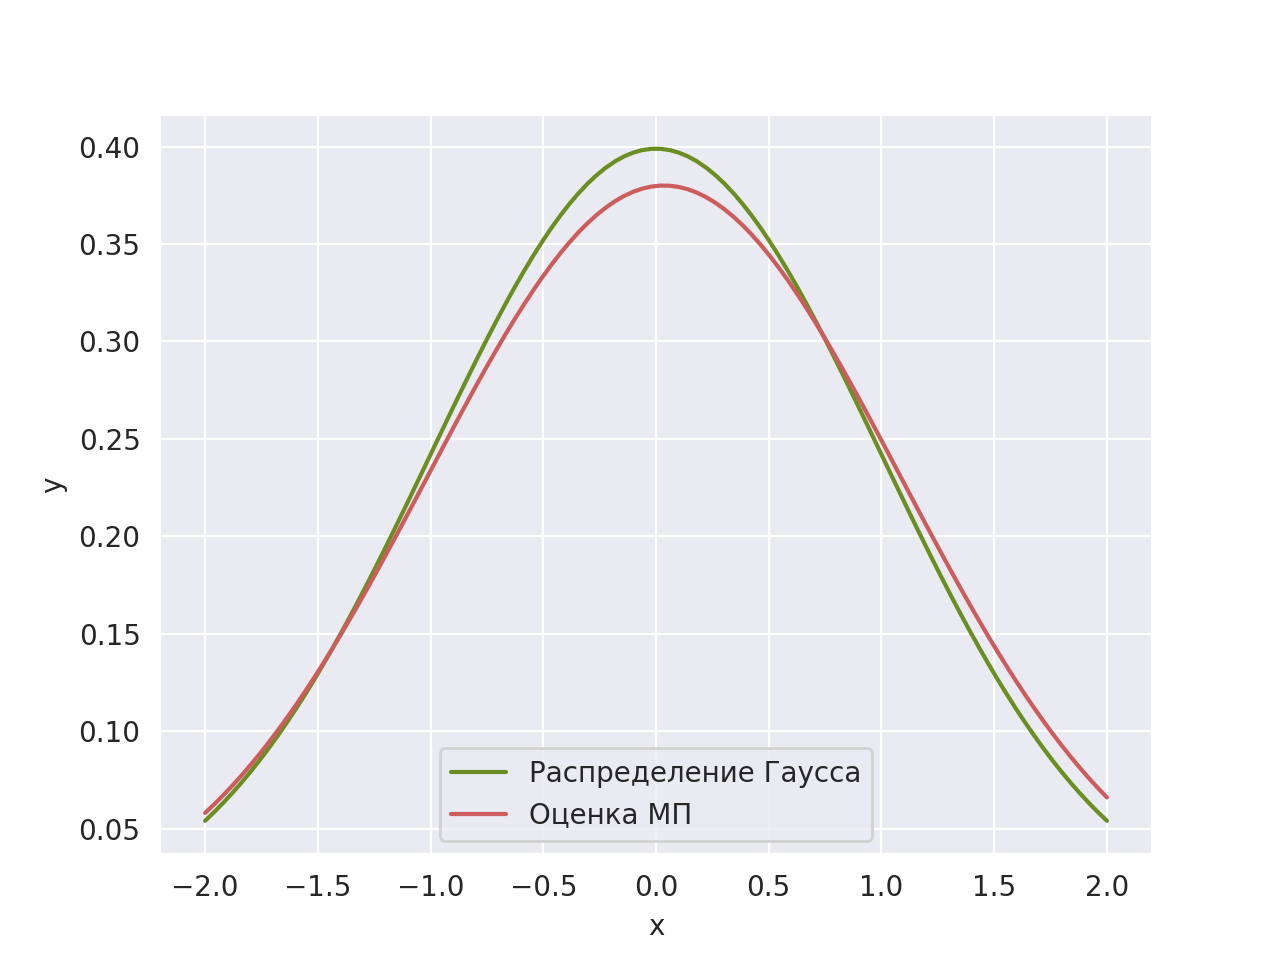
\includegraphics[width=13.5cm, height=10.cm]{mlm}
\label{pic_7:1}
\caption{Графики стандартного нормального распределения и распределения с параметрами, полученными методом МП}
\end{figure}

\newpage

$\chi^2_{1 - \alpha}(k - 1) = 26,296$
\begin{center}
    \begin{tabular}{ | c | c | c | c | c | c | c | c |}
        \hline
        $k = 16$ & $a_{i - 1}$ ; $a_{i}$ & $n_i$ & $\hat p_i$ & $n_i - n \hat p_i$ & $(n_i - n \hat p_i)^2/(n \hat p_i)$ \\ \hline
        1  &  -inf ; -3.50  &  0  &  0.0004  &  -0.04  &  0.04  \\ \hline
        2  &  -3.50 ; -2.96  &  0  &  0.0018  &  -0.18  &  0.18 \\ \hline
        3  &  -2.96 ; -2.42  &  1  &  0.0074  &  0.26  &  0.09  \\ \hline
        4  &  -2.42 ; -1.88  &  2  &  0.0241  &  -0.41  &  0.07 \\ \hline
        5  &  -1.88 ; -1.35  &  3  &  0.0604  &  -3.04  &  1.53 \\ \hline
        6  &  -1.35 ; -0.81  &  14  &  0.1169  &  2.31  &  0.46 \\ \hline
        7  &  -0.81 ; -0.27  &  22  &  0.1749  &  4.51  &  1.16 \\ \hline
        8  &  -0.27 ; 0.27  &  20  &  0.2023  &  -0.23  &  0.00 \\ \hline
        9  &  0.27 ; 0.81  &  15  &  0.1809  &  -3.09  &  0.53  \\ \hline
        10  &  0.81 ; 1.35  &  11  &  0.1251  &  -1.51  &  0.18 \\ \hline
        11  &  1.35 ; 1.88  &  7  &  0.0668  &  0.32  &  0.01   \\ \hline
        12  &  1.88 ; 2.42  &  4  &  0.0276  &  1.24  &  0.56   \\ \hline
        13  &  2.42 ; 2.96  &  1  &  0.0088  &  0.12  &  0.02   \\ \hline
        14  &  2.96 ; 3.50  &  0  &  0.0022  &  -0.22  &  0.22  \\ \hline
        15  &  3.50 ; inf  &  0  &  0.0005  &  -0.05  &  0.05   \\ \hline
        $\sum$ &  –––––––– &  100  &  1  & 0 & $\chi^2_{B}$ = 5.09 \\ \hline
    \end{tabular}
    \captionof{table}{Таблица вычислений $\chi^2_{B}$ при проверке гипотезы о нормальности распределения}
\end{center}

$\chi^2_{B} = 5.09 < 26.296 \approx \chi^2_{1 - \alpha}(k - 1)$ –– гипотеза принимается

%%%%%%%%%%%%%%%%%%%%%%%%%%%%%%%%%%%%%%%%%%

\section*{Вывод}
\addcontentsline{toc}{section}{Вывод}

\indent{\indent В случае нормального распределения оценка параметров распределения методом максимума правдоподобия эффективна, состоятельна, асимптотически нормальна. В ходе проверки гипотезы было получено значение $\chi^2_{B} = 5.09$, являющееся очень малым, и соответствующий ему уровень значимости равен $\alpha = 0.99$, что говорит об очень хорошем согласии гипотезы $H_0$ и полученных данных.}
%%%%%%%%%%%%%%%%%%%%%%%%%%%%%%%%%%%%%%%%%%

\newpage
\begin{thebibliography}{}
    \bibitem{ms_1}\textit{Амосова Н.Н., Куклин Б.А., Макарова С.Б., Максимов Ю.Д., Митрофанова Н.М., Полищук В.И., Шевляков Г.Л.} Вероятностные разделы математики. Учебник для бакалавров технических направлений. –– СПб.: Иван Федоров, 2001. –– 592 с.: илл. — ISBN 5-81940-050-X.
\end{thebibliography}


\end{document}{}